\documentclass[11pt]{beamer}
\usetheme{Pittsburgh}
\usepackage{xcolor}
\usepackage{pifont,enumitem}
\usepackage{etoolbox}
\usepackage{textpos}
\usepackage{capt-of}% or use the larger `caption` package
%\usepackage[pass]{geometry} 
\usepackage{multirow}
\usepackage{hhline} 
\usepackage{colortbl}
\usepackage{tikz}
\usetikzlibrary{trees,automata,positioning}
\usepackage{verbatim}
\usepackage{mathdots}

\setbeamertemplate{frametitle}{%
    \nointerlineskip%
    \usebeamerfont{frametitle}%
    \begin{beamercolorbox}[wd=\paperwidth,ht=1cm,sep=3pt]{frametitle}

        \includegraphics[height=1.2\baselineskip]{"VOUW logo-03"}
        \hfill\usebeamerfont{frametitle}\insertframetitle%

    \end{beamercolorbox}
}

\setbeamercolor{frametitle}{fg=red!45!yellow,bg=teal!75}
\setbeamercolor*{title}{fg=teal!75}
\usepackage{microtype}
\usepackage[utf8]{inputenc}

% import from STIX
\DeclareFontEncoding{LS1}{}{}
\DeclareFontSubstitution{LS1}{stix}{m}{n}
\DeclareFontFamily{LS1}{stixfrak}{\skewchar\font127 }
\DeclareFontShape{LS1}{stixfrak}{m}{n} {<-> stix-mathfrak}{}
\newcommand{\tplus}{\text{\usefont{LS1}{stixfrak}{m}{n}\symbol{"EB}}}
\newcommand{\tminus}{\text{\usefont{LS1}{stixfrak}{m}{n}\symbol{"EC}}}
%%%

\usepackage{amsmath}
\usepackage{amsfonts}
\usepackage{amssymb}
\usepackage{graphicx}
\usepackage[T1]{fontenc}
\usepackage{lmodern}
\usepackage{MnSymbol}

\setlist[itemize]{label={\color{red!45!yellow}\Pifont{pzd}{\char93}}}
\renewcommand{\mark}[1]{\textcolor{red!45!yellow}{\textbf{#1}}}
\renewcommand{\bold}[1]{\textcolor{teal}{\textbf{#1}}}

% Set the overall layout of the tree
\tikzstyle{level 1}=[level distance=3.0cm, sibling distance=1.3cm]
\tikzstyle{level 2}=[level distance=3.5cm, sibling distance=1.3cm]
\tikzstyle{level 3}=[level distance=3.5cm, sibling distance=1.3cm]

% Define styles for bags and leafs
\tikzstyle{l1} = [rectangle, text width=3em, text centered]
\tikzstyle{l2} = [rectangle, text width=5em, text centered]
\tikzstyle{l3} = [rectangle, text width=5em, text centered]

\author{Micky Faas}
\title{Pattern Mining on Matrices}
%\setbeamercovered{transparent} 
%\setbeamertemplate{navigation symbols}{} 
%\logo{} 
%\institute{} 
%\date{} 
%\subject{} 

\begin{document}
\beamertemplatenavigationsymbolsempty
\begin{frame}
\nointerlineskip%
\begin{columns}
\column{\dimexpr\paperwidth}
\centering % Center table


\includegraphics[width=0.4\paperwidth]{"VOUW logo-01"} 
\maketitle
\end{columns}
\end{frame}

%\begin{frame}
%\tableofcontents
%\end{frame}
%%%%%%%%%%

\begin{frame}{Overview}
With VOUW we propose a method of \textbf{mining patterns on matrices}. It encompasses:
\begin{itemize}
\item A theoretical framework
\item An optimization problem formulated using MDL
\item A heuristic algorithm.
\end{itemize}
\end{frame}

%%%%%%%%%%

\begin{frame}{Where is Waldo?}
\nointerlineskip%
\begin{columns}
\column{\dimexpr\paperwidth}
\centering
\includegraphics[width=\paperwidth]{"waldo"} 
\end{columns}
\end{frame}

%%%%%%%%%%

\begin{frame}{Informal problem}
Say we have some $M\times N$ matrix $A$, we want to discover and extract recurring structure.
Why?
\begin{itemize}
\item Data analysis
\item Distance metric for comparison
\item Clustering
\end{itemize}
\end{frame}


%%%%%%%%%%

\begin{frame}{Optimized Waldo}
\nointerlineskip%
\begin{columns}
\column{\dimexpr\paperwidth}
\centering
\includegraphics[width=\paperwidth]{"optimal waldo"} 
\end{columns}
\end{frame}

%%%%%%%%%%

\begin{frame}{Patterns and Instances}

\begin{tabular}{l l p{5cm}}
Term? & Form & Encodes... \\
\hline 
\textbf{Pattern} & Submatrix of $A$ & ...relative positions of elements \\
\textbf{Offset} & $(i,j)\in M\times N$ & ...position of entire pattern\\
\textbf{Instance} & $M\times N$ matrix & ...absolute positions of elements \\
\textbf{Instantiation} & $M\times N$ matrix & ...what pattern's instance should be at which index
\end{tabular}

%%%%%%%%%%%

\begin{align*}
\underbrace{
\begin{bmatrix}
1 & \cdot \\[-.2em]
\cdot & 1
\end{bmatrix}}_{\textsf{Pattern}},
\underbrace{
\begin{bmatrix}
\cdot & \cdot & \cdot & \cdot & \cdot & \cdot  \\[-.2em]
\cdot & \cdot & \cdot & \cdot & \cdot & \cdot  \\[-.2em]
\cdot & \cdot & 1 & \cdot & \cdot & \cdot  \\[-.2em]
\cdot & \cdot & \cdot & 1 & \cdot & \cdot  \\[-.2em]
\cdot & \cdot & \cdot & \cdot & \cdot & \cdot  \\[-.2em]
\cdot & \cdot & \cdot & \cdot & \cdot & \cdot  \\
\end{bmatrix}}_{\textsf{Instance with offset }(2,2)}
\end{align*}
\end{frame}

%%%%%%%%%%

\begin{frame}{Example}
\begin{align*}
A =
\overbrace{
\begin{bmatrix}
1 & \cdot & \cdot & \cdot & \cdot & 1  \\[-.2em]
\cdot & 1 & \cdot & \cdot & \cdot & \cdot \\[-.2em]
1 & \cdot & \cdot & \cdot & 1 & \cdot  \\[-.2em]
\cdot & 1 & \cdot & \cdot & \cdot & 1  \\[-.2em]
1 & \cdot & 1 & \cdot & \cdot & \cdot  \\[-.2em]
\cdot & 1 & \cdot & 1 & \cdot & \cdot  \\
\end{bmatrix}}^{\textsf{Original matrix}},
G = 
\overbrace{
\begin{bmatrix}
X & \cdot & \cdot & \cdot & \cdot & Y  \\[-.2em]
\cdot & \cdot & \cdot & \cdot & \cdot & \cdot  \\[-.2em]
X & \cdot & \cdot & \cdot & X & \cdot  \\[-.2em]
\cdot & \cdot & \cdot & \cdot & \cdot & \cdot  \\[-.2em]
X & \cdot & X & \cdot & \cdot & \cdot  \\[-.2em]
\cdot & \cdot & \cdot & \cdot & \cdot & \cdot  \\
\end{bmatrix}}^{\textsf{Instantiation}}\\
\overbrace{
H = \{
X =
\underbrace{
\begin{bmatrix}
1 & \cdot \\[-.2em]
\cdot & 1
\end{bmatrix}}_{\textsf{Pattern}},
Y =
\underbrace{
\begin{bmatrix}
1
\end{bmatrix}}_{\textsf{Pattern}}
\}}^{\textsf{Model}}
\end{align*}
\end{frame}

%%%%%%%%%%

\begin{frame}{Building Patterns}
We can construct complex patterns by repeatedly combining simpler ones. We use instances for this as they encode the position of one pattern relative to another.

\begin{align*}
\underbrace{
\begin{matrix}
X = \begin{bmatrix}
0
\end{bmatrix} \\[1.0em]
Y = \begin{bmatrix}
1
\end{bmatrix}
\end{matrix}}_{\textsf{Singleton patterns}}
\longrightarrow
\underbrace{\begin{matrix}
\bar{X} = \begin{bmatrix}
\cdot  & \cdot & \cdot \\
0 & \cdot & \cdot \\
\cdot & \cdot & \cdot \\
\end{bmatrix} \\[1.0em]
\bar{Y} = \begin{bmatrix}
\cdot  & \cdot & \cdot \\
\cdot  & \cdot & \cdot \\
\cdot & 1 & \cdot
\end{bmatrix}
\end{matrix}}_{\textsf{Instances}}
\longrightarrow
\bar{X}+\bar{Y} =
\underbrace{
\begin{bmatrix}
\cdot  & \cdot & \cdot \\
0  & \cdot & \cdot \\
\cdot & 1 & \cdot
\end{bmatrix}}_{\textsf{Matrix sum}}
\longrightarrow
\underbrace{
\begin{bmatrix}
0  & \cdot \\
\cdot & 1 
\end{bmatrix}}_{\textsf{New pattern}}
\end{align*}
\end{frame}

%%%%%%%%%%%

\begin{frame}{Model Space}
Idea: we inductively define the model space by starting with singletons for each element of $A$. Then we repeatedly merge instances until we finally obtain a pattern that equals $A$.
\begin{itemize}
\item At the beginning we have the completely underfit model
\item We end up with a completely overfit model
\end{itemize}
\bigskip
Everything in between is a possible solution, but \emph{we want the solution that describes $A$ best.}\\[1em]
For example $A=\begin{bmatrix}0 & 1 \\ 1 & 0\end{bmatrix}$: what is the space of possible solutions?
\end{frame}

%%%%%%%%%%%

\begin{frame}{2x2 Model Space Lattice}

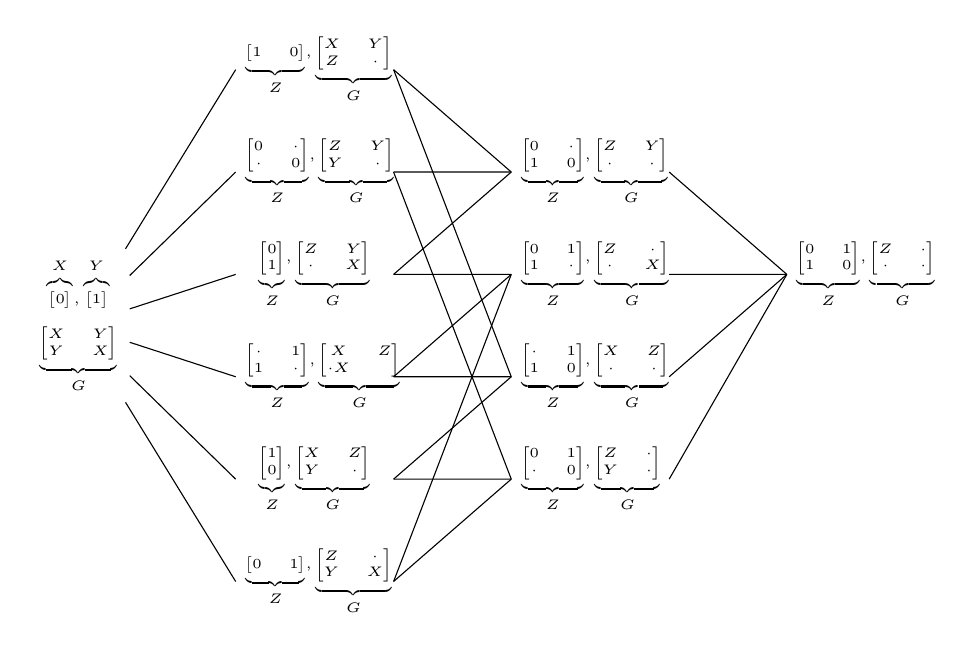
\begin{tikzpicture}[on grid, grow=right]
\node(R)[l1] {\tiny $\begin{matrix}\overbrace{\begin{bmatrix}0\end{bmatrix}}^{X},\overbrace{\begin{bmatrix}1\end{bmatrix}}^{Y}\\[1em]\underbrace{\begin{bmatrix}X & Y \\Y & X\end{bmatrix}}_{G}\end{matrix}$}
	child {
        node(F)[l2] {\tiny $\underbrace{\begin{bmatrix}0 & 1\end{bmatrix}}_{Z},\underbrace{\begin{bmatrix}Z & \cdot \\Y & X\end{bmatrix}}_{G}$}        
            edge from parent[draw=none] 
            (R) edge (F.west)
    }
    child {
        node(E)[l2] {\tiny $\underbrace{\begin{bmatrix}1 \\ 0\end{bmatrix}}_{Z},\underbrace{\begin{bmatrix}X & Z \\ Y & \cdot\end{bmatrix}}_{G}$}        
            child {
                node(J)[l3]
                    {\tiny $\underbrace{\begin{bmatrix}0 & 1 \\ \cdot & 0\end{bmatrix}}_{Z},\underbrace{\begin{bmatrix}Z & \cdot \\ Y & \cdot\end{bmatrix}}_{G}$}
                edge from parent 
            }
            edge from parent[draw=none] 
            (R) edge (E.west)
    }    
    child {
        node(D)[l2] {\tiny $\underbrace{\begin{bmatrix}\cdot & 1 \\ 1 & \cdot\end{bmatrix}}_{Z},\underbrace{\begin{bmatrix}X & Z \\ \cdot X\end{bmatrix}}_{G}$}        
            child {
                node(I)[l3]
                    {\tiny $\underbrace{\begin{bmatrix}\cdot & 1 \\ 1 & 0\end{bmatrix}}_{Z},\underbrace{\begin{bmatrix}X & Z \\ \cdot & \cdot\end{bmatrix}}_{G}$}
                edge from parent 
            }
            edge from parent[draw=none] 
            (R) edge (D.west)
    }    
    child {
        node(C)[l2] {\tiny $\underbrace{\begin{bmatrix}0 \\ 1\end{bmatrix}}_{Z},\underbrace{\begin{bmatrix}Z & Y \\\cdot & X\end{bmatrix}}_{G}$}        
            child {
                node(H)[l3]
                    {\tiny $\underbrace{\begin{bmatrix}0 & 1 \\ 1 & \cdot\end{bmatrix}}_{Z},\underbrace{\begin{bmatrix}Z & \cdot \\ \cdot & X\end{bmatrix}}_{G}$
                    }                    
                    	child {
                    		node(K)[l3] {\tiny $\underbrace{\begin{bmatrix}0 & 1 \\ 1 & 0\end{bmatrix}}_{Z},\underbrace{\begin{bmatrix}Z & \cdot \\ \cdot & \cdot\end{bmatrix}}_{G}$}
                    	}
                edge from parent 
            }
            edge from parent[draw=none] 
            (R) edge (C.west)
    }    
    child {
        node(B)[l2] {\tiny $\underbrace{\begin{bmatrix}0 & \cdot \\ \cdot & 0\end{bmatrix}}_{Z},\underbrace{\begin{bmatrix}Z & Y \\Y & \cdot\end{bmatrix}}_{G}$}        
            child {
                node(G)[l3]
                    {\tiny $\underbrace{\begin{bmatrix}0 & \cdot \\ 1 & 0\end{bmatrix}}_{Z},\underbrace{\begin{bmatrix}Z & Y \\ \cdot & \cdot\end{bmatrix}}_{G}$}
                edge from parent 
            }
            edge from parent[draw=none] 
            (R) edge (B.west)
    } 
    child {
        node(A)[l2] {\tiny $\underbrace{\begin{bmatrix}1 &0\end{bmatrix}}_{Z},\underbrace{\begin{bmatrix}X & Y \\Z & \cdot\end{bmatrix}}_{G}$}        
        	edge from parent[draw=none] 
            (R) edge (A.west)
    };
\draw(F.east)--(H.west);
\draw(F.east)--(J.west);
\draw(B.east)--(J.west);
\draw(C.east)--(G.west);
\draw(D.east)--(H.west);
\draw(E.east)--(I.west);
\draw(A.east)--(G.west);
\draw(A.east)--(I.west);
\draw(G.east)--(K.west);
\draw(I.east)--(K.west);
\draw(J.east)--(K.west);
\end{tikzpicture}
\end{frame}

%%%%%%%%%%%%%

\begin{frame}{Worst-case complexity}

How complex is this lattice? Very complex!\\
Idea: pick two instances to combine $MN-1$ times.
\begin{align*}
\displaystyle\prod^{MN-2}_{n=0} \binom{MN-n}{2} = \displaystyle\prod^{MN-2}_{n=0} \frac{MN-n}{2(MN-n-2)!} = \frac{(MN)!(MN-1)!}{2^{MN-1}} .
\end{align*}\\[3em]
We will need to use heuristics.

\end{frame}

%%%%%%%%%%%%%

\begin{frame}{Optimization using MDL}

Idea: the best solution is a balance of model and instantiation complexity. We use two-part MDL:

$$
\underbrace{L(H)}_{\textsf{Model}} + \underbrace{L(A|H)}_{\textsf{Data given model}}
$$

In this case:

\begin{align*}
L\left(
\underbrace{
\overbrace{
\begin{bmatrix}
1 & \cdot \\[-.2em]
\cdot & 1
\end{bmatrix}}^{\textsf{Pattern}},
\overbrace{
\begin{bmatrix}
1
\end{bmatrix}}^{\textsf{Pattern}}
}_{\textsf{Model}}
\right)
+
L\left(
\underbrace{ 
\overbrace{
\begin{matrix}
X & \cdot & \cdot & \cdot & \cdot & Y  \\[-.2em]
\cdot & \cdot & \cdot & \cdot & \cdot & \cdot  \\[-.2em]
X & \cdot & \cdot & \cdot & X & \cdot  \\[-.2em]
\cdot & \cdot & \cdot & \cdot & \cdot & \cdot  \\[-.2em]
X & \cdot & X & \cdot & \cdot & \cdot  \\[-.2em]
\cdot & \cdot & \cdot & \cdot & \cdot & \cdot  \\
\end{matrix}}}^{\textsf{Instantiation Matrix}}_{\textsf{Data given model}}
\right)
\end{align*}
\end{frame}

%%%%%%%%%%%%%

\begin{frame}{Motivation}

Why does this work? MDL is founded on these principles:\\[1em]
\begin{description}
\item[Kolmogorov Complexity] of given data is the shortest computer program to produce that data.
\item[Occam's Razor]. Given competing hypotheses, pick the one with the fewest assumptions.
\item[No-hypercompression theorem]. Data with no inherent structure, cannot be compressed.
\item[Kraft Inequality]. One-to-one correspondence between code lengths and probabilities.
\end{description}

\end{frame}

%%%%%%%%%%%%%

\begin{frame}{A Simple Algorithm}

Idea: look at $A$ once to build an instantiation matrix $G$. Make a model $H$ using only singleton patterns, one for each possible value in $A$.\\[1em]

Then we constantly refine our description by merging instances to form patterns. Once we merge instances, we never reconsider (greedy approach).\\[1em]

\tiny
$$
\begin{matrix}\overbrace{\begin{bmatrix}0\end{bmatrix}}^{X},\overbrace{\begin{bmatrix}1\end{bmatrix}}^{Y}\\[1em]\underbrace{\begin{bmatrix}X & Y \\Y & X\end{bmatrix}}_{G}\end{matrix}\ \longrightarrow
\ \underbrace{\begin{bmatrix}1 &0\end{bmatrix}}_{Z},\underbrace{\begin{bmatrix}X & Y \\Z & \cdot\end{bmatrix}}_{G}
\ \longrightarrow
\ \underbrace{\begin{bmatrix}0 & \cdot \\ 1 & 0\end{bmatrix}}_{Z},\underbrace{\begin{bmatrix}Z & Y \\ \cdot & \cdot\end{bmatrix}}_{G}
$$

\end{frame}

%%%%%%%%%%%%%

\begin{frame}{Candidates}

Which pair of instances do we combine? We will first derive a list of candidates from the instantiation matrix:

$$
\underbrace{
\begin{bmatrix}
\cellcolor{red!45!yellow} X & Y & X & Y & \cellcolor{red!45!yellow}X & X  \\[-.2em]
\cellcolor{red!45!yellow}X & \cellcolor{red!45!yellow}Y & X & X & Y & \cellcolor{red!45!yellow}Y  \\[-.2em]
Y & \cellcolor{red!45!yellow}Y & \cellcolor{red!45!yellow}X & X & X & Y  \\[-.2em]
X & X & X & \cellcolor{red!45!yellow}Y & X & X  \\[-.2em]
\cellcolor{red!45!yellow}X & X & X & X & X & X  \\[-.2em]
X & \cellcolor{red!45!yellow}Y & X & X & X & Y  \\
\end{bmatrix}}_{\textsf{Instantiation matrix}}
\longrightarrow
\underbrace{
\begin{matrix}
\cellcolor{red!45!yellow} X &   \\[-.2em]
 & \cellcolor{red!45!yellow}Y  \\[-.2em]
\end{matrix}}_{\textsf{Candidate}}
$$
\bigskip
The candidate that minimizes the MDL equation best is picked.

\end{frame}

%%%%%%%%%%%%%

\begin{frame}{Adjacency}

We constrain the idea of the last slides by only looking at \textbf{adjacent} instances.

$$
\begin{matrix}
\ddots & \vdots & \vdots & \vdots & \vdots & \vdots & \iddots \\[-.2em]
\cdots & \cdot & \cdot & \cdot & \cdot & \cdot & \cdots \\[-.2em]
\cdots & \cdot & \cellcolor{teal!75} & \cellcolor{teal!75} & \cellcolor{teal!75} & \cellcolor{red!45!yellow}\cdot & \cdots \\[-.2em]
\cdots & \cdot & \cellcolor{teal!75} & \cellcolor{red!45!yellow}\cdot & \cellcolor{teal!75} & \cellcolor{red!45!yellow}\cdot & \cdots \\[-.2em]
\cdots & \cdot & \cellcolor{teal!75} & \cellcolor{red!45!yellow}\cdot & \cellcolor{red!45!yellow}\cdot & \cellcolor{red!45!yellow}\cdot & \cdots \\[-.2em]
\cdots & \cellcolor{red!45!yellow}\cdot & \cellcolor{red!45!yellow}\cdot & \cellcolor{red!45!yellow}\cdot & \cellcolor{red!45!yellow}\cdot & \cellcolor{red!45!yellow}\cdot & \cdots \\[-.2em]
\cdots & \cdot & \cdot & \cdot & \cdot & \cdot & \cdots \\[-.4em]
\iddots & \vdots & \vdots & \vdots & \vdots & \vdots & \ddots
\end{matrix}
$$
This gives two benefits: (1) visits all candidates just once, (2) reduces candidate space.

\end{frame}


%%%%%%%%%%%%%

\begin{frame}{A Simple Algorithm (2)}

This simple algorithm gives an acceptable complexity:
\begin{itemize}
\item Each iteration (find candidates and merge best) is (almost) linear.
\item $MN-1$ iterations worst-case, but we need only a fraction in any practical case.
\end{itemize}
\bigskip
However:
\begin{itemize}
\item Greedy approach sometimes gives completely wrong results.
\item No tolerance to noise.
\end{itemize}

\end{frame}

%%%%%%%%%%%%%

\begin{frame}{Open Problems}
A `wish list' for the future:
\begin{itemize}
\item Actual data and use-cases (!)
\item Noise robustness.
\item Multi-instance candidates (more than 2).
\item Hierarchical encoding of patterns.
\item Improvement of the current (prequential) encoding.
\end{itemize}
\end{frame}

%%%%%%%%%%%%%

\begin{frame}{Here is Waldo}
\nointerlineskip%
\begin{columns}
\column{\dimexpr\paperwidth}
\centering
\includegraphics[width=\paperwidth]{"here is waldo"} 
\end{columns}
\end{frame}
\end{document}